\documentclass[aspectratio=169,10pt]{ctexbeamer}

\usetheme{Madrid}
\usecolortheme{default}
\setbeamertemplate{navigation symbols}{}

\usepackage{amsmath,amssymb,mathtools,bm}
\usepackage{array,booktabs,multirow}
\usepackage{graphicx}
\usepackage{tikz}
\usetikzlibrary{arrows.meta,calc}


\newcommand{\ds}{\displaystyle}
\newcommand{\topic}[1]{\textcolor{blue!70!black}{\textbf{#1}}}
\newcommand{\sep}{\vspace{0.35em}}

% Unified Yingxing Beamer footer and visual style.
\newcommand{\huayinglogo}{assets/logo1.jpg}
\newcommand{\huayingslogan}{英行培优，成绩无忧；英行相伴，刮目相看}

\setbeamersize{text margin left=8mm,text margin right=8mm}
\setbeamerfont{frametitle}{size=\large}
\setbeamercolor{structure}{fg=blue!70!black}
\setbeamercolor{frametitle}{bg=blue!75!black,fg=white}
\setbeamercolor{block title}{bg=blue!10,fg=black}
\setbeamercolor{block body}{bg=blue!2,fg=black}
\setbeamercolor{author in head/foot}{bg=blue!8,fg=black}
\setbeamercolor{title in head/foot}{bg=blue!8,fg=black}

\setbeamertemplate{footline}{%
  \leavevmode%
  \hbox{%
    \begin{beamercolorbox}[wd=.12\paperwidth,ht=3.8ex,dp=1.2ex,center]{author in head/foot}%
      \includegraphics[height=2.9ex]{\huayinglogo}%
    \end{beamercolorbox}%
    \begin{beamercolorbox}[wd=.76\paperwidth,ht=3.8ex,dp=1.2ex,center]{title in head/foot}%
      \scriptsize \huayingslogan
    \end{beamercolorbox}%
    \begin{beamercolorbox}[wd=.12\paperwidth,ht=3.8ex,dp=1.2ex,right]{author in head/foot}%
      \scriptsize \insertframenumber/\inserttotalframenumber\hspace*{1em}
    \end{beamercolorbox}%
  }%
}

\title{导数的概念与应用初步}
\subtitle{知识梳理 + 题组重排版}
\author{}
\date{}

\begin{document}

\begin{frame}
  \titlepage
\end{frame}

\begin{frame}[t]{导数概念 1: 平均变化率}
\small
\begin{block}{知识点 1 平均变化率}
对于函数 $y=f(x)$，当自变量由 $x_0$ 变到 $x_0+\Delta x$ 时，
\[
\Delta y=f(x_0+\Delta x)-f(x_0),\qquad
\frac{\Delta y}{\Delta x}=\frac{f(x_0+\Delta x)-f(x_0)}{\Delta x}.
\]
比值 $\dfrac{\Delta y}{\Delta x}$ 称为函数从 $x_0$ 到 $x_0+\Delta x$ 的平均变化率。
\end{block}
\end{frame}

\begin{frame}[t]{导数概念 2: 瞬时变化率与导数定义}
\small
\begin{block}{知识点 2 瞬时变化率与导数}
当 $\Delta x\to 0$ 时，若
\[
\frac{f(x_0+\Delta x)-f(x_0)}{\Delta x}\to k,
\]
则称常数 $k$ 为函数 $f(x)$ 在 $x=x_0$ 处的瞬时变化率，也就是导数：
\[
f'(x_0)=\lim_{\Delta x\to 0}\frac{f(x_0+\Delta x)-f(x_0)}{\Delta x}.
\]
\end{block}

\begin{alertblock}{理解要点}
导数本质上刻画的是函数在某一点附近的“局部变化快慢”。
\end{alertblock}
\end{frame}

\begin{frame}[t]{导数概念 2: 几何意义与切线方程}
\small
\begin{columns}[T,totalwidth=\textwidth]
\begin{column}{0.55\textwidth}
\begin{block}{知识点 3 割线斜率与切线斜率}
过点
$A(x_0,f(x_0))$ 与 $B(x_0+\Delta x,f(x_0+\Delta x))$ 的割线斜率为
\[
\frac{f(x_0+\Delta x)-f(x_0)}{\Delta x}.
\]
当点 $B$ 沿曲线趋近于点 $A$ 时，割线极限位置就是曲线在点 $A$ 处的切线。
\end{block}

\begin{block}{知识点 4 导数的几何意义}
\[
f'(x_0)=k
\]
表示曲线 $y=f(x)$ 在点 $(x_0,f(x_0))$ 处切线的斜率。

切线方程：
\[
y-f(x_0)=f'(x_0)(x-x_0).
\]
\end{block}
\end{column}
\begin{column}{0.45\textwidth}
\centering
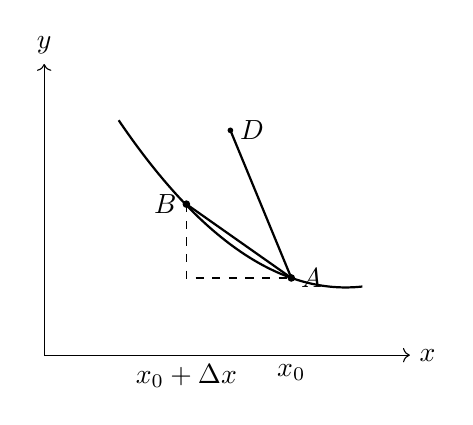
\begin{tikzpicture}[scale=0.86]
  \draw[->] (0,0)--(5.4,0) node[right] {$x$};
  \draw[->] (0,0)--(0,4.3) node[above] {$y$};
  \draw[thick,domain=1.1:4.7,samples=120,smooth] plot(\x,{0.22*(\x-4.45)^2+1.0});
  \coordinate (A) at (3.65,1.14);
  \coordinate (B) at (2.1,2.23);
  \coordinate (C) at (2.1,1.14);
  \coordinate (D) at (2.75,3.32);
  \draw[dashed] (B)--(C)--(A);
  \draw[thick] (A)--(B);
  \draw[thick] (A)--(D);
  \fill (A) circle (1.6pt) node[right] {$A$};
  \fill (B) circle (1.6pt) node[left] {$B$};
  \fill (D) circle (1.2pt) node[right] {$D$};
  \node[below] at (3.65,0) {$x_0$};
  \node[below] at (2.1,0) {$x_0+\Delta x$};
\end{tikzpicture}
\end{column}
\end{columns}
\end{frame}

\begin{frame}[t]{导数运算: 常用公式}
\small
\topic{常用求导公式}

\renewcommand{\arraystretch}{1.18}
\begin{center}
\begin{tabular}{|>{\centering\arraybackslash}m{0.28\linewidth}|>{\centering\arraybackslash}m{0.42\linewidth}|}
\hline
原函数 & 导函数 \\
\hline
$c$ & $0$ \\
\hline
$x^\alpha$ & $\alpha x^{\alpha-1}$ \\
\hline
$\sin x$ & $\cos x$ \\
\hline
$\cos x$ & $-\sin x$ \\
\hline
$a^x$ & $a^x\ln a$ \\
\hline
$e^x$ & $e^x$ \\
\hline
$\log_a x$ & $\dfrac{1}{x\ln a}$ \\
\hline
$\ln x$ & $\dfrac{1}{x}$ \\
\hline
\end{tabular}
\end{center}
\end{frame}

\begin{frame}[t]{导数运算: 法则与提醒}
\small
\topic{导数运算法则}
\begin{align*}
[f(x)\pm g(x)]'&=f'(x)\pm g'(x),\\
[f(x)g(x)]'&=f'(x)g(x)+f(x)g'(x),\\
\left[\frac{f(x)}{g(x)}\right]'&=
\frac{f'(x)g(x)-f(x)g'(x)}{g^2(x)}.
\end{align*}

\sep
\topic{复合函数求导}
\[
y=f(u),\quad u=g(x)
\]
则
\[
\frac{dy}{dx}=\frac{dy}{du}\cdot\frac{du}{dx}.
\]

\sep
\begin{alertblock}{提醒}
做单调性、极值、最值问题时，求导只是起点，关键是结合定义域与导数符号表。
\end{alertblock}
\end{frame}

\begin{frame}[t]{函数性质 1: 导数与单调性}
\small
\begin{block}{导数与单调性}
设函数 $f(x)$ 在区间 $(a,b)$ 上可导，则
\[
f'(x)>0\Rightarrow f(x)\text{ 在 }(a,b)\text{ 上单调递增},
\]
\[
f'(x)<0\Rightarrow f(x)\text{ 在 }(a,b)\text{ 上单调递减},
\]
\[
f'(x)=0\Rightarrow f(x)\text{ 在 }(a,b)\text{ 上为常数函数}.
\]
\end{block}
\end{frame}

\begin{frame}[t]{函数性质 2: 极值判定}
\small
\begin{block}{极值判定}
求极值的一般步骤：
\begin{enumerate}
  \item 确定定义域并求导；
  \item 解方程 $f'(x)=0$；
  \item 列导数符号表；
  \item 根据左右两侧单调性的变化判定极大值、极小值。
\end{enumerate}
\end{block}
\end{frame}

\begin{frame}[t]{函数性质 3: 最值问题}
\small
\begin{block}{最值问题}
若 $f(x)$ 在 $[a,b]$ 上连续，在 $(a,b)$ 内可导，则最值通常由两部分比较得到：
\[
\text{端点函数值}\quad \text{与}\quad \text{区间内极值}.
\]
\end{block}
\end{frame}

\begin{frame}[t]{微专题 4: 切线问题 1}
\large
\begin{block}{例 1}
[2024 全国甲卷] 设函数
\[
f(x)=\frac{e^x+2\sin x}{1+x^2},
\]
则曲线 $y=f(x)$ 在点 $(0,1)$ 处的切线与两坐标轴所围成三角形的面积为
\[
\underline{\hspace{3cm}}.
\]
\end{block}
\end{frame}

\begin{frame}[t,allowframebreaks]{解析: 微专题 4 切线问题 1}
\tiny
\begin{block}{解题步骤}
先求切线斜率。因为
\[
f(x)=\frac{e^x+2\sin x}{1+x^2},
\]
由商的求导法则，
\[
f'(x)=\frac{(e^x+2\cos x)(1+x^2)-2x(e^x+2\sin x)}{(1+x^2)^2}.
\]
代入 $x=0$，得
\[
f(0)=1,\qquad f'(0)=1+2=3.
\]
所以曲线在 $(0,1)$ 处的切线方程为
\[
y-1=3(x-0),\quad 即\quad y=3x+1.
\]
该直线与 $y$ 轴交于 $(0,1)$，与 $x$ 轴交于 $\left(-\frac13,0\right)$。
因此所围三角形的两条直角边长分别为 $1$ 与 $\frac13$，面积为
\[
S=\frac12\cdot1\cdot\frac13=\frac16.
\]
\end{block}
\end{frame}

\begin{frame}[t]{微专题 4: 切线问题 2}
\large
\begin{block}{例 2}
若直线 $y=kx+1$ 为常数，是曲线 $y=\ln x+1$ 和曲线 $y=ae^x+1$ 的公切线，
求实数 $a$ 的值。
\end{block}
\end{frame}

\begin{frame}[t,allowframebreaks]{解析: 微专题 4 切线问题 2}
\tiny
\begin{block}{解题步骤}
设直线先与 $y=\ln x+1$ 相切，切点横坐标为 $t>0$。该曲线导数为 $\frac1x$，
所以切线斜率
\[
k=\frac1t.
\]
切线方程为
\[
y-(\ln t+1)=\frac1t(x-t),
\]
整理得
\[
y=\frac1t x+\ln t.
\]
它又等于题设直线 $y=kx+1$，比较截距得
\[
\ln t=1,\quad t=e,\quad k=\frac1e.
\]
\end{block}
\end{frame}

\begin{frame}[t,allowframebreaks]{解析: 微专题 4 切线问题 2 续}
\tiny
\begin{block}{解题步骤}
再设它与 $y=ae^x+1$ 相切，切点横坐标为 $s$。导数为 $ae^x$，故斜率条件给出
\[
ae^s=\frac1e.
\]
切线方程为
\[
y-(ae^s+1)=ae^s(x-s).
\]
由于 $ae^s=\frac1e$，其截距为
\[
1+\frac1e-\frac{s}{e}.
\]
该截距应等于 $1$，所以 $s=1$。代回 $ae^s=\frac1e$，得
\[
ae=\frac1e,\qquad a=e^{-2}.
\]
\end{block}
\end{frame}

\begin{frame}[t]{微专题 4: 切线问题 3}
\large
\begin{block}{例 3}
[2025 河北保定二模] 已知直线
\[
y=x+m\quad (m>0)
\]
是圆
\[
C:(x+1)^2+y^2=2
\]
与曲线
\[
y=\frac12\ln(2x-1)+a
\]
的公切线，则
\[
a+m=\underline{\hspace{3cm}}.
\]
\end{block}
\end{frame}

\begin{frame}[t,allowframebreaks]{解析: 微专题 4 切线问题 3}
\tiny
\begin{block}{解题步骤}
直线 $y=x+m$ 写成一般式为
\[
x-y+m=0.
\]
它与圆 $(x+1)^2+y^2=2$ 相切，所以圆心 $(-1,0)$ 到直线的距离等于半径 $\sqrt2$：
\[
\frac{|(-1)-0+m|}{\sqrt{1^2+(-1)^2}}=\sqrt2.
\]
于是
\[
|m-1|=2.
\]
又 $m>0$，故
\[
m=3.
\]
\end{block}
\end{frame}

\begin{frame}[t,allowframebreaks]{解析: 微专题 4 切线问题 3 续}
\tiny
\begin{block}{解题步骤}
曲线
\[
y=\frac12\ln(2x-1)+a
\]
的导数为
\[
y'=\frac12\cdot\frac2{2x-1}=\frac1{2x-1}.
\]
公切线斜率为 $1$，所以
\[
\frac1{2x-1}=1,\quad x=1.
\]
此时曲线上点为 $(1,a)$，切线为
\[
y-a=1(x-1),\quad 即\quad y=x+a-1.
\]
与 $y=x+m=x+3$ 比较，得
\[
a-1=3,\quad a=4.
\]
所以
\[
a+m=4+3=7.
\]
\end{block}
\end{frame}

\begin{frame}[t]{微专题 4: 单调性}
\large
\begin{block}{训练 1}
[2025 江苏泰州四模] 已知函数
\[
f(x)=\sin(2x-2)-e^{1-x}+e^{x-1}+2\quad (x\in\mathbb{R}),
\]
若
\[
f(2a^2)+f(1-a)<4,
\]
求实数 $a$ 的取值范围。
\end{block}
\end{frame}

\begin{frame}[t,allowframebreaks]{解析: 微专题 4 单调性}
\tiny
\begin{block}{解题步骤}
将函数关于 $x=1$ 平移。令
\[
F(t)=f(1+t)-2.
\]
由题设函数得
\[
F(t)=\sin 2t+e^t-e^{-t}.
\]
显然 $F(-t)=-F(t)$，即 $F$ 为奇函数。

再看单调性：
\[
F'(t)=2\cos2t+e^t+e^{-t}=2(\cos2t+\cosh t).
\]
因为 $\cosh t\ge1$，且 $\cos2t\ge-1$，并且二者不可能同时取到使和为 $0$ 的情形，
所以
\[
F'(t)>0.
\]
故 $F$ 在 $\mathbb R$ 上严格递增。
\end{block}
\end{frame}

\begin{frame}[t,allowframebreaks]{解析: 微专题 4 单调性 续}
\tiny
\begin{block}{解题步骤}
原不等式为
\[
f(2a^2)+f(1-a)<4,
\]
即
\[
F(2a^2-1)+F(-a)<0.
\]
由奇函数性质 $F(-a)=-F(a)$，得
\[
F(2a^2-1)<F(a).
\]
由于 $F$ 严格递增，等价于
\[
2a^2-1<a.
\]
解得
\[
2a^2-a-1<0,\qquad -\frac12<a<1.
\]
\end{block}
\end{frame}

\begin{frame}[t]{微专题 4: 极值与综合}
\large
\begin{block}{训练 2}
[2023 北京卷] 设函数
\[
f(x)=x-x^3e^{ax+b},
\]
曲线 $y=f(x)$ 在点 $(1,f(1))$ 处的切线方程为 $y=-x+1$。
\begin{enumerate}
  \item 求 $a,b$ 的值；
  \item 设函数 $g(x)=f'(x)$，求 $g(x)$ 的单调区间；
  \item 求 $f(x)$ 的极值点个数。
\end{enumerate}
\end{block}
\end{frame}

\begin{frame}[t,allowframebreaks]{解析: 微专题 4 极值与综合}
\tiny
\begin{block}{第 1 问}
切线方程为 $y=-x+1$，切点横坐标为 $1$，所以
\[
f(1)=0,\qquad f'(1)=-1.
\]
又
\[
f(1)=1-e^{a+b},
\]
故
\[
a+b=0.
\]
对
\[
f(x)=x-x^3e^{ax+b}
\]
求导：
\[
f'(x)=1-\left(3x^2+ax^3\right)e^{ax+b}.
\]
代入 $x=1$ 且 $a+b=0$，
\[
f'(1)=1-(3+a)=-a-2.
\]
由 $f'(1)=-1$，得
\[
a=-1,\qquad b=1.
\]
\end{block}
\begin{block}{第 2、3 问}
此时
\[
f(x)=x-x^3e^{1-x},\quad g(x)=f'(x)=1+x^2(x-3)e^{1-x}.
\]
继续求导：
\[
g'(x)=-x(x^2-6x+6)e^{1-x}.
\]
由于 $e^{1-x}>0$，只需讨论
\[
-x(x^2-6x+6)=-x\{(x-3)^2-3\}.
\]
临界点为
\[
x=0,\quad x=3-\sqrt3,\quad x=3+\sqrt3.
\]
列符号可得：$g$ 的增区间为
\[
(-\infty,0),\quad (3-\sqrt3,3+\sqrt3),
\]
减区间为
\[
(0,3-\sqrt3),\quad (3+\sqrt3,+\infty).
\]
又 $g(x)\to-\infty\ (x\to-\infty)$，$g(0)=1$，$g(1)=-1$，$g(3)=1$，
故 $g(x)=0$ 有三个实根。即 $f'(x)=0$ 有三个变号零点，所以 $f(x)$ 的极值点个数为
\[
3.
\]
\end{block}
\end{frame}

\begin{frame}[t]{微专题 5: 函数零点 1}
\large
\begin{block}{例 1}
已知函数
\[
f(x)=ax^3-3x^2+1,
\]
若 $f(x)$ 存在唯一零点 $x_0$，且 $x_0>0$，求 $a$ 的取值范围。
\end{block}
\end{frame}

\begin{frame}[t,allowframebreaks]{解析: 微专题 5 函数零点 1}
\tiny
\begin{block}{解题步骤}
考虑
\[
f(x)=ax^3-3x^2+1.
\]
若 $a=0$，则 $f(x)=-3x^2+1$ 有两个零点，不合题意。下面设 $a\ne0$。

三次方程
\[
ax^3-3x^2+1=0
\]
的判别式为
\[
\Delta=27(4-a^2).
\]
当 $|a|<2$ 时有三个不同实根；当 $|a|=2$ 时有重根但仍有两个不同实根；
只有当
\[
|a|>2
\]
时，方程只有一个实根。

还需判断这个唯一零点是否为正。若 $a>2$，则
\[
f(0)=1>0,\qquad \lim_{x\to+\infty}f(x)=+\infty.
\]
并且在正半轴上唯一可能的极小点为 $x=\frac2a$，此时
\[
f\left(\frac2a\right)=1-\frac4{a^2}>0.
\]
所以 $x>0$ 上无零点，唯一零点在负半轴。
\end{block}
\end{frame}

\begin{frame}[t,allowframebreaks]{解析: 微专题 5 函数零点 1 续}
\tiny
\begin{block}{解题步骤}
若 $a<-2$，则
\[
f(0)=1>0,\qquad \lim_{x\to+\infty}f(x)=-\infty,
\]
由连续性知正半轴上存在零点；又总共只有一个实根，所以该唯一零点为正。

综上，
\[
a<-2.
\]
\end{block}
\end{frame}

\begin{frame}[t]{微专题 5: 函数零点 2}
\large
\begin{block}{例 2}
[2025 广州三模] 已知函数
\[
f(x)=ax^2+(a-2)x-\ln x \quad (x>0).
\]
\begin{enumerate}
  \item 当 $a=2$ 时，求与 $f(x)$ 图象相切，且垂直于直线 $x+3y=0$ 的直线方程；
  \item 若 $f(x)$ 有两个零点，求实数 $a$ 的取值范围。
\end{enumerate}
\end{block}
\end{frame}

\begin{frame}[t,allowframebreaks]{解析: 微专题 5 函数零点 2}
\tiny
\begin{block}{第 1 问}
当 $a=2$ 时，
\[
f(x)=2x^2-\ln x,\qquad f'(x)=4x-\frac1x.
\]
直线 $x+3y=0$ 的斜率为 $-\frac13$，与它垂直的直线斜率为 $3$。
设切点横坐标为 $t>0$，则
\[
f'(t)=3,\quad 即\quad 4t-\frac1t=3.
\]
化为
\[
4t^2-3t-1=0,
\]
得
\[
t=1\quad (t>0).
\]
切点为
\[
(1,f(1))=(1,2).
\]
所以所求切线方程为
\[
y-2=3(x-1),\quad 即\quad y=3x-1.
\]
\end{block}
\begin{block}{第 2 问}
零点方程
\[
ax^2+(a-2)x-\ln x=0
\]
可整理为
\[
a(x^2+x)=2x+\ln x.
\]
由于 $x>0$，$x^2+x>0$，故
\[
a=A(x):=\frac{2x+\ln x}{x^2+x}.
\]
求导得
\[
A'(x)=-\frac{(2x+1)(x+\ln x-1)}{x^2(x+1)^2}.
\]
函数 $x+\ln x-1$ 在 $(0,+\infty)$ 上严格递增，且在 $x=1$ 处为 $0$。
所以 $A(x)$ 在 $(0,1)$ 上递增，在 $(1,+\infty)$ 上递减，最大值
\[
A(1)=1.
\]
又
\[
\lim_{x\to0^+}A(x)=-\infty,\qquad \lim_{x\to+\infty}A(x)=0^+.
\]
因此直线 $y=a$ 与 $A(x)$ 的图象有两个交点，当且仅当
\[
0<a<1.
\]
\end{block}
\end{frame}

\begin{frame}[t]{微专题 5: 函数零点 3}
\large
\begin{columns}[T,totalwidth=\textwidth]
\begin{column}{0.58\textwidth}
\begin{block}{自测题}
已知函数
\[
f(x)=\ln x-ax.
\]
\begin{enumerate}
  \item 当 $a=2$ 时，求函数 $f(x)$ 的单调区间；
  \item 设 $g(x)=f(x)+1$，讨论函数 $g(x)$ 的零点个数。
\end{enumerate}
\end{block}
\end{column}
\begin{column}{0.42\textwidth}
\centering
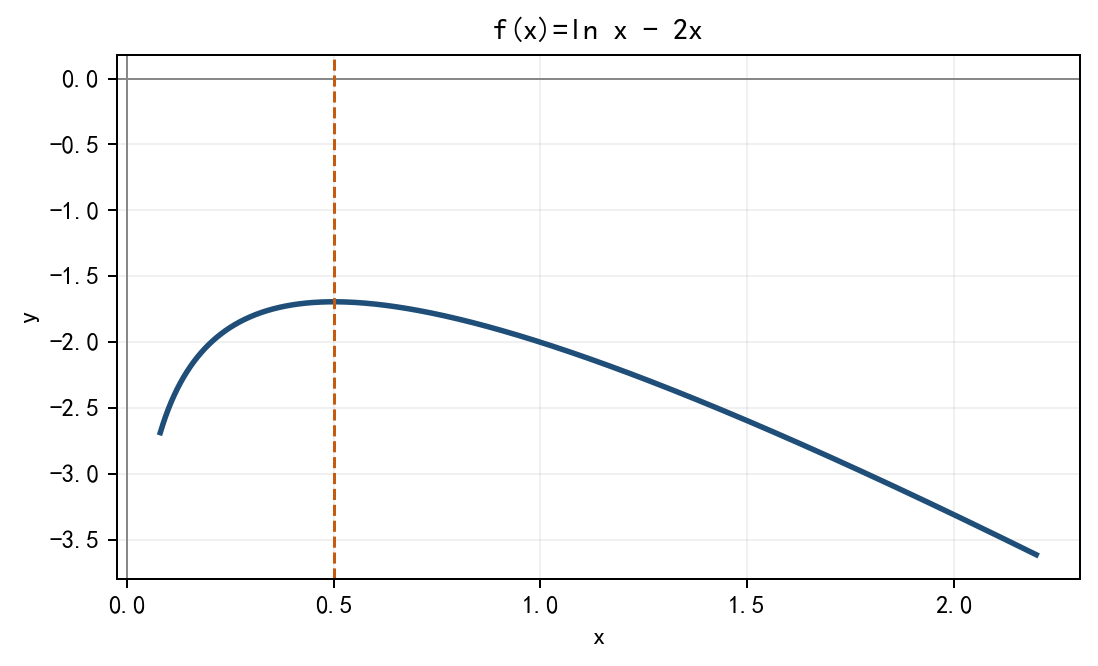
\includegraphics[width=\linewidth]{assets/graph_lnx_minus_2x.png}
\end{column}
\end{columns}
\end{frame}

\begin{frame}[t,allowframebreaks]{解析: 微专题 5 函数零点 3}
\tiny
\begin{block}{第 1 问}
当 $a=2$ 时，
\[
f(x)=\ln x-2x,\qquad f'(x)=\frac1x-2=\frac{1-2x}{x}.
\]
因为定义域为 $(0,+\infty)$，所以 $x>0$，导数符号由 $1-2x$ 决定。
于是
\[
f'(x)>0\quad (0<x<\tfrac12),\qquad f'(x)<0\quad (x>\tfrac12).
\]
故单调递增区间为
\[
\left(0,\frac12\right),
\]
单调递减区间为
\[
\left(\frac12,+\infty\right).
\]
\end{block}
\begin{block}{第 2 问}
\[
g(x)=\ln x-ax+1,\qquad g'(x)=\frac1x-a.
\]
若 $a\le0$，则 $g'(x)>0$，且
\[
\lim_{x\to0^+}g(x)=-\infty,\qquad \lim_{x\to+\infty}g(x)=+\infty,
\]
所以有 $1$ 个零点。

若 $a>0$，则 $g'(x)=0$ 的唯一解为 $x=\frac1a$，此处为最大值点，且
\[
g\left(\frac1a\right)=\ln\frac1a-1+1=-\ln a.
\]
当 $0<a<1$ 时，最大值 $-\ln a>0$，两端极限均为 $-\infty$，故有 $2$ 个零点；
当 $a=1$ 时，最大值为 $0$，故有 $1$ 个零点；
当 $a>1$ 时，最大值小于 $0$，故无零点。
\end{block}
\end{frame}

\begin{frame}[t]{微专题 5: 隐零点问题}
\large
\begin{block}{例 3}
已知函数
\[
f(x)=ax^2-ax-x\ln x,
\]
且 $f(x)\ge 0$。
\begin{enumerate}
  \item 求 $a$；
  \item 证明：$f(x)$ 存在唯一的极大值点 $x_0$，且
  \[
  e^{-2}<f(x_0)<2^{-2}.
  \]
\end{enumerate}
\end{block}
\end{frame}

\begin{frame}[t,allowframebreaks]{解析: 微专题 5 隐零点问题}
\tiny
\begin{block}{第 1 问}
题中函数默认在 $x>0$ 上讨论。因为
\[
f(x)=ax^2-ax-x\ln x=x\{a(x-1)-\ln x\},
\]
且 $x>0$，所以 $f(x)\ge0$ 等价于
\[
a(x-1)\ge\ln x\quad (x>0).
\]
当 $x>1$ 时，除以正数 $x-1$ 得
\[
a\ge \frac{\ln x}{x-1}.
\]
令 $x\to1^+$，右端趋于 $1$，所以必须 $a\ge1$。

当 $0<x<1$ 时，除以负数 $x-1$，不等号反向：
\[
a\le \frac{\ln x}{x-1}.
\]
令 $x\to1^-$，右端也趋于 $1$，所以必须 $a\le1$。
因此
\[
a=1.
\]
\end{block}
\begin{block}{第 2 问}
此时
\[
f(x)=x^2-x-x\ln x,\qquad f'(x)=2x-2-\ln x.
\]
设
\[
h(x)=2x-2-\ln x.
\]
则
\[
h'(x)=2-\frac1x.
\]
所以 $h$ 在 $(0,\frac12)$ 上递减，在 $(\frac12,+\infty)$ 上递增。
又
\[
\lim_{x\to0^+}h(x)=+\infty,\quad h\left(\frac12\right)=\ln2-1<0,\quad h(1)=0,
\]
故 $h(x)=0$ 在 $(0,\frac12)$ 上有唯一根 $x_0$，并且另一个根为 $1$。
由 $f'$ 的符号变化可知，$x_0$ 是唯一极大值点，$1$ 是极小值点。
\end{block}
\end{frame}

\begin{frame}[t,allowframebreaks]{解析: 微专题 5 隐零点问题 续}
\tiny
\begin{block}{极大值估计}
由 $h(x_0)=0$ 得
\[
\ln x_0=2x_0-2.
\]
所以
\[
f(x_0)=x_0^2-x_0-x_0\ln x_0
=x_0^2-x_0-x_0(2x_0-2)
=x_0(1-x_0).
\]
先估计 $x_0$ 的范围。因为
\[
h(e^{-2})=2e^{-2}>0,\qquad h\left(\frac12\right)=\ln2-1<0,
\]
且 $h$ 在 $(0,\frac12)$ 上递减，所以
\[
e^{-2}<x_0<\frac12.
\]
于是
\[
f(x_0)=x_0(1-x_0)<\frac12\cdot\frac12=\frac14=2^{-2}.
\]
\end{block}
\end{frame}

\begin{frame}[t,allowframebreaks]{解析: 微专题 5 隐零点问题 续 2}
\tiny
\begin{block}{极大值估计}
另一方面，由 $\ln x_0=2x_0-2$ 可得 $x_0=e^{2x_0-2}$，所以
\[
f(x_0)=x_0(1-x_0)=e^{-2}\,e^{2x_0}(1-x_0).
\]
令 $\psi(x)=2x+\ln(1-x)$，则在 $0<x<\frac12$ 上
\[
\psi'(x)=2-\frac1{1-x}>0,\qquad \psi(0)=0.
\]
故 $e^{2x_0}(1-x_0)>1$，从而
\[
f(x_0)>e^{-2}.
\]
综上，
\[
e^{-2}<f(x_0)<2^{-2}.
\]
\end{block}
\end{frame}

\begin{frame}[t]{微专题 6: 不等式恒成立 1}
\large
\begin{block}{例 1}
[2025 华中师大一附中模拟] 已知函数
\[
f(x)=(x-a)\ln x.
\]
\begin{enumerate}
  \item 若 $x=1$ 为 $f(x)$ 的极值点，求 $a$；
  \item 当 $x\ge 1$ 时，若 $f(x)\ge x+a-1$ 恒成立，求 $a$ 的取值范围。
\end{enumerate}
\end{block}
\end{frame}

\begin{frame}[t,allowframebreaks]{解析: 微专题 6 不等式恒成立 1}
\tiny
\begin{block}{第 1 问}
\[
f(x)=(x-a)\ln x,\qquad f'(x)=\ln x+\frac{x-a}{x}=\ln x+1-\frac ax.
\]
若 $x=1$ 为极值点，必要条件是
\[
f'(1)=0.
\]
代入得
\[
0+1-a=0,\qquad a=1.
\]
此时 $f'(x)=\ln x+1-\frac1x$，且 $f''(x)=\frac1x+\frac1{x^2}>0$，
所以 $x=1$ 确为极小值点。
\end{block}
\begin{block}{第 2 问}
对 $x\ge1$，不等式
\[
(x-a)\ln x\ge x+a-1
\]
整理为
\[
x\ln x-x+1\ge a(\ln x+1).
\]
因为 $x\ge1$ 时 $\ln x+1>0$，故等价于
\[
a\le R(x):=\frac{x\ln x-x+1}{\ln x+1}.
\]
要对一切 $x\ge1$ 恒成立，就需
\[
a\le \min_{x\ge1}R(x).
\]
求导：
\[
R'(x)=\frac{x(\ln x)^2+x-1}{x(\ln x+1)^2}.
\]
当 $x\ge1$ 时，分子非负，故 $R$ 递增。于是
\[
\min_{x\ge1}R(x)=R(1)=0.
\]
因此
\[
a\le0.
\]
\end{block}
\end{frame}

\begin{frame}[t]{微专题 6: 不等式恒成立 2}
\large
\begin{block}{例 2}
设函数
\[
f(x)=a\ln x+\frac{1-a}{2}x^2-bx\quad (a\ne 1),
\]
曲线 $y=f(x)$ 在点 $(1,f(1))$ 处的切线斜率为 $0$。
\begin{enumerate}
  \item 求 $b$；
  \item 若存在 $x_0\ge 1$，使得
  \[
  f(x_0)<\frac{a}{a-1},
  \]
  求 $a$ 的取值范围。
\end{enumerate}
\end{block}
\end{frame}

\begin{frame}[t,allowframebreaks]{解析: 微专题 6 不等式恒成立 2}
\tiny
\begin{block}{第 1 问}
\[
f'(x)=\frac ax+(1-a)x-b.
\]
切线斜率为 $0$，即
\[
f'(1)=a+(1-a)-b=0.
\]
所以
\[
b=1.
\]
\end{block}
\begin{block}{第 2 问}
代入 $b=1$，得
\[
f(x)=a\ln x+\frac{1-a}{2}x^2-x.
\]
要求存在 $x_0\ge1$ 使
\[
f(x_0)<\frac a{a-1}.
\]
先讨论 $f$ 在 $[1,+\infty)$ 上的最小值。求导并分解：
\[
f'(x)=\frac ax+(1-a)x-1
=\frac{(x-1)((1-a)x-a)}x.
\]
若 $a\le \frac12$，则在 $x\ge1$ 上有 $f'(x)\ge0$，最小值为
\[
f(1)=\frac{1-a}{2}-1=-\frac{a+1}{2}.
\]
于是存在所求 $x_0$ 等价于
\[
-\frac{a+1}{2}<\frac a{a-1}.
\]
化简得
\[
a\in(-1-\sqrt2,\,-1+\sqrt2),
\]
再与 $a\le\frac12$ 结合，仍为
\[
-1-\sqrt2<a<-1+\sqrt2.
\]
\end{block}
\end{frame}

\begin{frame}[t,allowframebreaks]{解析: 微专题 6 不等式恒成立 2 续}
\tiny
\begin{block}{继续讨论}
若 $\frac12<a<1$，则
\[
x=\frac a{1-a}>1
\]
是 $f$ 在 $[1,+\infty)$ 上的极小值点。将它代入并与 $\frac a{a-1}$ 比较：
\[
f\left(\frac a{1-a}\right)-\frac a{a-1}
=\frac{a\{-a+2(a-1)\ln\frac a{1-a}\}}{2(a-1)}.
\]
因为 $\frac12<a<1$ 时 $\ln\frac a{1-a}>0$，且 $a-1<0$，故大括号内为负数；
分母 $2(a-1)$ 也为负数，因此上式为正。也就是说
\[
\min f(x)>\frac a{a-1},
\]
所以不存在满足条件的 $x_0$。
\end{block}
\end{frame}

\begin{frame}[t,allowframebreaks]{解析: 微专题 6 不等式恒成立 2 续 2}
\tiny
\begin{block}{继续讨论}
若 $a>1$，则 $1-a<0$，当 $x\to+\infty$ 时，
\[
f(x)=a\ln x+\frac{1-a}{2}x^2-x\to-\infty.
\]
因此一定存在充分大的 $x_0$，使
\[
f(x_0)<\frac a{a-1}.
\]

综上所述，
\[
a\in(-1-\sqrt2,\,-1+\sqrt2)\cup(1,+\infty).
\]
\end{block}
\end{frame}

\begin{frame}[t]{微专题 6: 不等式恒成立 3}
\large
\begin{block}{例 3}
[2024 新课标 I 卷] 已知函数
\[
f(x)=\ln\frac{x}{2-x}+ax+b(x-1)^3.
\]
\begin{enumerate}
  \item 若 $b=0$，且 $f'(x)\ge 0$，求 $a$ 的最小值；
  \item 证明：曲线 $y=f(x)$ 是中心对称图形；
  \item 当 $1<x<2$ 时，若 $f(x)$ 的值域是 $(-2,+\infty)$，求 $b$ 的取值范围。
\end{enumerate}
\end{block}
\end{frame}

\begin{frame}[t,allowframebreaks]{解析: 微专题 6 不等式恒成立 3}
\tiny
\begin{block}{第 1 问}
当 $b=0$ 时，
\[
f(x)=\ln\frac{x}{2-x}+ax.
\]
定义域为 $0<x<2$。求导：
\[
f'(x)=\frac1x+\frac1{2-x}+a=\frac2{x(2-x)}+a.
\]
因为
\[
x(2-x)=1-(x-1)^2\le1,
\]
所以
\[
\frac2{x(2-x)}\ge2.
\]
因此要使 $f'(x)\ge0$ 对定义域内任意 $x$ 恒成立，只需且必须
\[
2+a\ge0.
\]
所以 $a$ 的最小值为
\[
-2.
\]
\end{block}
\begin{block}{第 2 问}
令 $x=1+t$，则 $t\in(-1,1)$。有
\[
f(1+t)=\ln\frac{1+t}{1-t}+a(1+t)+bt^3,
\]
\[
f(1-t)=\ln\frac{1-t}{1+t}+a(1-t)-bt^3.
\]
相加得
\[
f(1+t)+f(1-t)=2a.
\]
这说明曲线上关于横坐标 $x=1$ 对称的两点，其纵坐标和恒为 $2a$，
故曲线 $y=f(x)$ 关于点
\[
(1,a)
\]
中心对称。
\end{block}
\end{frame}

\begin{frame}[t,allowframebreaks]{解析: 微专题 6 不等式恒成立 3 续}
\tiny
\begin{block}{第 3 问}
若在 $1<x<2$ 上值域为 $(-2,+\infty)$，由于
\[
\lim_{x\to1^+}f(x)=a,
\]
下确界为 $-2$ 且不取到，必须有
\[
a=-2.
\]
令
\[
t=x-1\quad (0<t<1).
\]
此时
\[
f(x)+2=\ln\frac{1+t}{1-t}-2t+bt^3.
\]
要使值域为 $(-2,+\infty)$，需
\[
\ln\frac{1+t}{1-t}-2t+bt^3>0\quad (0<t<1),
\]
且当 $t\to0^+$ 时趋于 $0$。
\end{block}
\end{frame}

\begin{frame}[t,allowframebreaks]{解析: 微专题 6 不等式恒成立 3 续 2}
\tiny
\begin{block}{第 3 问}
利用展开
\[
\ln\frac{1+t}{1-t}=2\left(t+\frac{t^3}{3}+\frac{t^5}{5}+\cdots\right),
\]
可知
\[
\ln\frac{1+t}{1-t}-2t=\frac23t^3+\frac25t^5+\cdots.
\]
所以必要条件为
\[
b+\frac23\ge0,\quad 即\quad b\ge-\frac23.
\]
当 $b\ge-\frac23$ 时，
\[
\ln\frac{1+t}{1-t}-2t+bt^3
\ge \left(\frac23+b\right)t^3>0\quad (0<t<1),
\]
故条件也充分。因此
\[
b\ge-\frac23.
\]
\end{block}
\end{frame}

\begin{frame}[t]{微专题 6: 自测题}
\large
\begin{block}{训练}
[2025 西南“3+3+3”一诊] 已知函数
\[
f(x)=\ln(2x+1)-4\sin x.
\]
\begin{enumerate}
  \item 求曲线在点 $(0,f(0))$ 处的切线方程；
  \item 若存在 $x\in\left[0,\frac{\pi}{2}\right]$，使得 $f(x)\ge a$ 成立，求 $a$ 的取值范围。
\end{enumerate}
\end{block}
\end{frame}

\begin{frame}[t,allowframebreaks]{解析: 微专题 6 自测题}
\tiny
\begin{block}{第 1 问}
\[
f(x)=\ln(2x+1)-4\sin x,
\]
所以
\[
f'(x)=\frac2{2x+1}-4\cos x.
\]
在 $x=0$ 处，
\[
f(0)=0,\qquad f'(0)=2-4=-2.
\]
故切线方程为
\[
y-0=-2(x-0),\quad 即\quad y=-2x.
\]
\end{block}
\begin{block}{第 2 问}
题意为存在 $x\in[0,\frac\pi2]$ 使 $f(x)\ge a$，等价于
\[
a\le \max_{0\le x\le\pi/2}f(x).
\]
下面求最大值。对 $x\in[0,\frac\pi2]$，
\[
\ln(2x+1)\le2x,
\]
且
\[
\sin x\ge \frac{2x}{\pi}.
\]
于是
\[
f(x)=\ln(2x+1)-4\sin x
\le 2x-\frac{8x}{\pi}\le0.
\]
当 $x=0$ 时，$f(0)=0$，所以最大值为 $0$。
因此
\[
a\le0.
\]
\end{block}
\end{frame}

\begin{frame}[t]{高分提能一: 零点与极值点证明 1}
\large
\begin{block}{典型例题 1}
[2025 福建龙岩三模] 已知函数
\[
f(x)=x^2+a\ln(x+1).
\]
\begin{enumerate}
  \item 当 $a=-4$ 时，求 $f(x)$ 的极小值；
  \item 若 $f(x)$ 存在唯一的极值点 $x_0$，证明
  \[
  f(x_0)+x_0^2\le 0.
  \]
\end{enumerate}
\end{block}
\end{frame}

\begin{frame}[t,allowframebreaks]{解析: 高分提能一 典型例题 1}
\tiny
\begin{block}{第 1 问}
当 $a=-4$ 时，
\[
f(x)=x^2-4\ln(x+1),\qquad x>-1.
\]
求导：
\[
f'(x)=2x-\frac4{x+1}
=\frac{2x(x+1)-4}{x+1}
=\frac{2(x+2)(x-1)}{x+1}.
\]
在定义域 $(-1,+\infty)$ 内，只有临界点 $x=1$。当 $-1<x<1$ 时，$f'(x)<0$；
当 $x>1$ 时，$f'(x)>0$。所以 $x=1$ 为极小值点，
\[
f_{\min}=f(1)=1-4\ln2.
\]
\end{block}
\begin{block}{第 2 问}
\[
f'(x)=2x+\frac a{x+1}
=\frac{2x(x+1)+a}{x+1}.
\]
因为 $x>-1$，分母恒正，极值点由
\[
2x(x+1)+a=0
\]
决定。若 $f$ 存在唯一极值点 $x_0$，则可推出 $x_0\ge0$，且
\[
a=-2x_0(x_0+1).
\]
代入原式：
\[
f(x_0)+x_0^2
=2x_0^2+a\ln(x_0+1)
=2x_0^2-2x_0(x_0+1)\ln(x_0+1).
\]
只需证
\[
x_0\le (x_0+1)\ln(x_0+1).
\]
令 $u=x_0+1\ge1$，该式等价于
\[
u-1\le u\ln u,
\]
即
\[
\ln u\ge1-\frac1u,
\]
这是 $\ln u$ 的基本不等式，成立。故
\[
f(x_0)+x_0^2\le0.
\]
\end{block}
\end{frame}

\begin{frame}[t]{高分提能一: 零点与极值点证明 2}
\large
\begin{block}{典型例题 2}
已知函数
\[
f(x)=(x-1)\ln x-x-1.
\]
证明：
\begin{enumerate}
  \item $f(x)$ 存在唯一的极值点；
  \item 方程 $f(x)=0$ 有且仅有两个实根，且两个实根互为倒数。
\end{enumerate}
\end{block}
\end{frame}

\begin{frame}[t,allowframebreaks]{解析: 高分提能一 典型例题 2}
\tiny
\begin{block}{第 1 问}
定义域为 $x>0$。
\[
f(x)=(x-1)\ln x-x-1.
\]
求导：
\[
f'(x)=\ln x+\frac{x-1}{x}-1=\ln x-\frac1x.
\]
再求导：
\[
f''(x)=\frac1x+\frac1{x^2}>0.
\]
所以 $f'(x)$ 在 $(0,+\infty)$ 上严格递增。又
\[
\lim_{x\to0^+}f'(x)=-\infty,\qquad \lim_{x\to+\infty}f'(x)=+\infty,
\]
故 $f'(x)=0$ 有唯一解，且 $f'$ 在该点左右变号。因此 $f(x)$ 存在唯一的极值点。
\end{block}
\begin{block}{第 2 问}
由
\[
\lim_{x\to0^+}f(x)=+\infty,\qquad f(1)=-2,\qquad \lim_{x\to+\infty}f(x)=+\infty,
\]
并结合上一问“先减后增”的单调结构，可知方程 $f(x)=0$ 有且仅有两个实根。

若 $r$ 是一个实根，则
\[
(r-1)\ln r-r-1=0,
\]
即
\[
(r-1)\ln r=r+1.
\]
计算
\[
f\left(\frac1r\right)
=\left(\frac1r-1\right)\ln\frac1r-\frac1r-1
=\frac{(r-1)\ln r-(r+1)}r=0.
\]
所以若 $r$ 是根，则 $\frac1r$ 也是根。两个根只有两个，因此它们互为倒数。
\end{block}
\end{frame}

\begin{frame}[t]{高分提能二: 含 $\ln x$、$e^x$ 的不等式 1}
\large
\begin{block}{例 1}
设函数
\[
f(x)=e^{2x}-a\ln x.
\]
\begin{enumerate}
  \item 讨论 $f'(x)$ 的零点个数；
  \item 证明：当 $a>0$ 时，
  \[
  f(x)\ge 2a+a\ln\frac{2}{a}.
  \]
\end{enumerate}
\end{block}
\end{frame}

\begin{frame}[t,allowframebreaks]{解析: 高分提能二 例 1}
\tiny
\begin{block}{第 1 问}
定义域为 $x>0$。
\[
f'(x)=2e^{2x}-\frac ax.
\]
方程 $f'(x)=0$ 等价于
\[
2xe^{2x}=a.
\]
令
\[
H(x)=2xe^{2x}\quad (x>0).
\]
则
\[
H'(x)=2e^{2x}(1+2x)>0,
\]
所以 $H$ 在 $(0,+\infty)$ 上严格递增，且
\[
\lim_{x\to0^+}H(x)=0,\qquad \lim_{x\to+\infty}H(x)=+\infty.
\]
因此：
\[
a\le0 \text{ 时 } f'(x) \text{ 无零点};\qquad
a>0 \text{ 时 } f'(x) \text{ 有唯一零点}.
\]
\end{block}
\begin{block}{第 2 问}
当 $a>0$ 时，设 $f'(x)$ 的唯一零点为 $x_0$，则
\[
a=2x_0e^{2x_0}.
\]
由于 $f'$ 由负变正，$x_0$ 为 $f$ 的最小值点。于是
\[
f(x)\ge f(x_0)=e^{2x_0}-a\ln x_0
=\frac a{2x_0}-a\ln x_0.
\]
又
\[
\ln\frac2a=\ln\frac1{x_0e^{2x_0}}=-\ln x_0-2x_0.
\]
故
\[
f(x_0)-\left(2a+a\ln\frac2a\right)
=a\left(\frac1{2x_0}+2x_0-2\right)
=a\cdot\frac{(2x_0-1)^2}{2x_0}\ge0.
\]
所以
\[
f(x)\ge 2a+a\ln\frac2a.
\]
\end{block}
\end{frame}

\begin{frame}[t]{高分提能二: 含 $\ln x$、$e^x$ 的不等式 2}
\large
\begin{columns}[T,totalwidth=\textwidth]
\begin{column}{0.57\textwidth}
\begin{block}{自测题}
[2022 全国甲卷] 已知函数
\[
f(x)=\frac{e^x}{x}-\ln x+x-a.
\]
\begin{enumerate}
  \item 若 $f(x)\ge 0$，求 $a$ 的取值范围；
  \item 证明：若 $f(x)$ 有两个零点 $x_1,x_2$，则 $x_1x_2<1$。
\end{enumerate}
\end{block}
\end{column}
\begin{column}{0.43\textwidth}
\centering
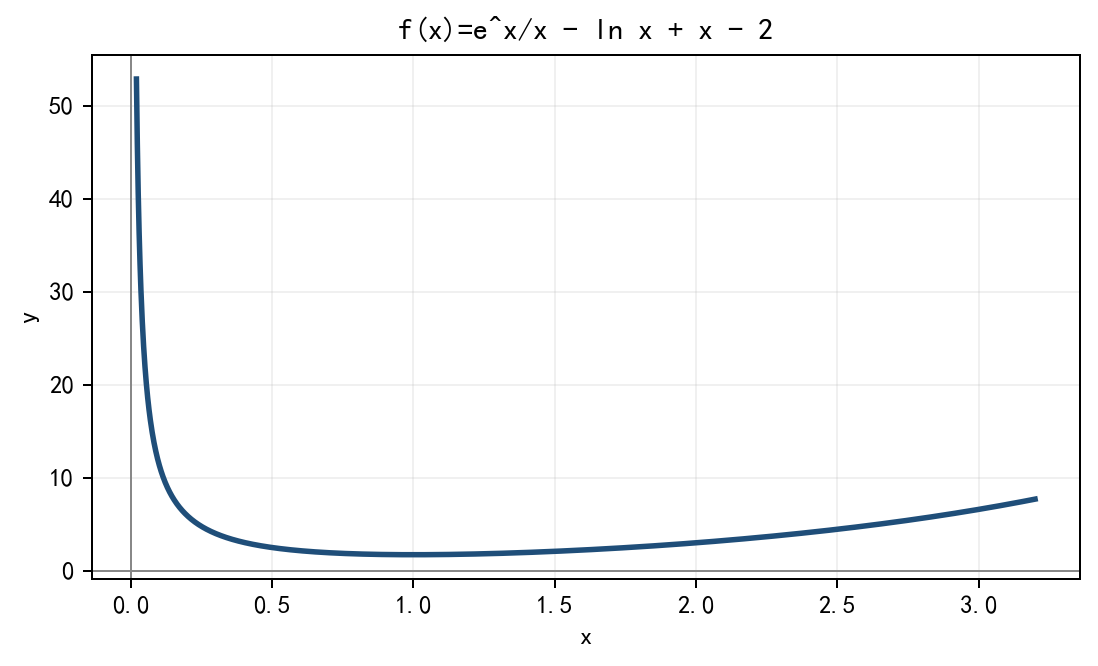
\includegraphics[width=\linewidth]{assets/graph_exp_over_x.png}
\end{column}
\end{columns}
\end{frame}

\begin{frame}[t,allowframebreaks]{解析: 高分提能二 自测题}
\tiny
\begin{block}{第 1 问}
令
\[
\phi(x)=\frac{e^x}{x}-\ln x+x\quad (x>0),
\]
则
\[
f(x)=\phi(x)-a.
\]
要求 $f(x)\ge0$ 对一切 $x>0$ 成立，等价于
\[
a\le \min_{x>0}\phi(x).
\]
求导：
\[
\phi'(x)=\frac{e^x(x-1)}{x^2}-\frac1x+1
=\frac{(x-1)(e^x+x)}{x^2}.
\]
由于 $e^x+x>0$，所以 $\phi$ 在 $(0,1)$ 上递减，在 $(1,+\infty)$ 上递增。
因此最小值为
\[
\phi(1)=e.
\]
故
\[
a\le e.
\]
\end{block}
\begin{block}{第 2 问}
若 $f$ 有两个零点 $x_1<x_2$，则
\[
\phi(x_1)=\phi(x_2)=a.
\]
由 $\phi$ 的单调性，必有
\[
x_1<1<x_2.
\]
对 $0<x<1$，可验证
\[
\phi\left(\frac1x\right)>\phi(x).
\]
若反设 $x_1x_2\ge1$，则 $x_2\ge\frac1{x_1}$。又 $\phi$ 在 $(1,+\infty)$ 上递增，所以
\[
\phi(x_2)\ge \phi\left(\frac1{x_1}\right)>\phi(x_1),
\]
这与 $\phi(x_1)=\phi(x_2)$ 矛盾。因此
\[
x_1x_2<1.
\]
\end{block}
\end{frame}

\begin{frame}[t]{高分提能三: 导数与数列交汇 1}
\large
\begin{block}{类型 1}
[2025 湖北武汉模拟] 已知函数
\[
f(x)=xe^{x-1}-a.
\]
\begin{enumerate}
  \item 若 $a\in\mathbb{R}$，讨论 $f(x)$ 的零点个数；
  \item 若 $a$ 为正整数，记 $f(x)$ 的唯一零点为 $x_n$，证明数列 $\{x_n\}$ 为递增数列。
\end{enumerate}
\end{block}
\end{frame}

\begin{frame}[t,allowframebreaks]{解析: 高分提能三 类型 1}
\tiny
\begin{block}{第 1 问}
方程 $f(x)=0$ 等价于
\[
xe^{x-1}=a.
\]
令
\[
h(x)=xe^{x-1}.
\]
则
\[
h'(x)=e^{x-1}(x+1).
\]
因为 $e^{x-1}>0$，所以 $h$ 在 $(-\infty,-1)$ 上递减，在 $(-1,+\infty)$ 上递增。
并且
\[
h(-1)=-e^{-2},\qquad h(0)=0,
\]
\[
\lim_{x\to-\infty}h(x)=0^-,\qquad \lim_{x\to+\infty}h(x)=+\infty.
\]
据此可得零点个数：
\[
\begin{cases}
0,&a<-e^{-2},\\
1,&a=-e^{-2},\\
2,&-e^{-2}<a<0,\\
1,&a=0,\\
1,&a>0.
\end{cases}
\]
\end{block}
\begin{block}{第 2 问}
若 $a=n$ 为正整数，则唯一零点 $x_n$ 满足
\[
x_ne^{x_n-1}=n.
\]
此时 $x_n>0$。而 $h(x)=xe^{x-1}$ 在 $(0,+\infty)$ 上严格递增。
若 $n_1<n_2$，则
\[
h(x_{n_1})=n_1<n_2=h(x_{n_2}),
\]
由 $h$ 的严格递增性得
\[
x_{n_1}<x_{n_2}.
\]
所以数列 $\{x_n\}$ 为递增数列。
\end{block}
\end{frame}

\begin{frame}[t]{高分提能三: 导数与数列交汇 2}
\large
\begin{block}{类型 2}
[2025 四川德阳二模节选] 已知数列 $\{a_n\}$ 的前 $n$ 项和为 $S_n$，满足
\[
S_{n+1}=3S_n-2n+4,\qquad a_1=4.
\]
\begin{enumerate}
  \item 求数列 $\{a_n\}$ 的通项公式；
  \item 令
  \[
  f(x)=a_1x+a_2x^2+\cdots+a_nx^n,
  \]
  讨论 $f'(1)$ 与 $\dfrac{8n^2+11n-3}{4}$ 的大小关系。
\end{enumerate}
\end{block}
\end{frame}

\begin{frame}[t,allowframebreaks]{解析: 高分提能三 类型 2}
\tiny
\begin{block}{第 1 问}
由
\[
S_{n+1}=3S_n-2n+4
\]
观察非齐次项，设
\[
S_n=C\cdot3^{n-1}+\alpha n+\beta.
\]
代入递推式，比较 $n$ 的系数和常数项，得
\[
\alpha=1,\qquad \beta=-\frac32.
\]
再由 $S_1=4$，
\[
C+1-\frac32=4,\quad C=\frac92.
\]
故
\[
S_n=\frac92\cdot3^{n-1}+n-\frac32.
\]
于是
\[
a_n=S_n-S_{n-1}=3^n+1\quad (n\ge2),
\]
且 $a_1=4=3^1+1$，所以
\[
a_n=3^n+1.
\]
\end{block}
\begin{block}{第 2 问}
\[
f'(1)=\sum_{k=1}^n k a_k
=\sum_{k=1}^n k(3^k+1).
\]
利用公式
\[
\sum_{k=1}^n k3^k=\frac{3-(n+1)3^{n+1}+n3^{n+2}}{(1-3)^2}
=\frac{(2n-1)3^{n+1}+3}{4},
\]
以及
\[
\sum_{k=1}^n k=\frac{n(n+1)}2,
\]
得
\[
f'(1)=\frac{(2n-1)3^{n+1}+2n^2+2n+3}{4}.
\]
与 $\frac{8n^2+11n-3}{4}$ 比较，$n=1$ 时相等；当 $n\ge2$ 时，指数项 $(2n-1)3^{n+1}$ 明显大于对应二次项，故
\[
f'(1)>\frac{8n^2+11n-3}{4}.
\]
\end{block}
\end{frame}

\begin{frame}[t]{高分提能四: 导数与三角函数结合 1}
\large
\begin{columns}[T,totalwidth=\textwidth]
\begin{column}{0.58\textwidth}
\begin{block}{例 1}
已知函数
\[
f(x)=-\sin x+kx.
\]
\begin{enumerate}
  \item 若 $f(x)$ 在 $\mathbb{R}$ 上单调，求 $k$ 的取值范围；
  \item 若
  \[
  g(x)=\frac{k^2}{6}x^3+x+\sin x,
  \]
  证明：$k$ 可以取无数个值，使得每个 $k$ 的取值下，$g(x)$ 都恰有三个不同零点。
\end{enumerate}
\end{block}
\end{column}
\begin{column}{0.42\textwidth}
\centering
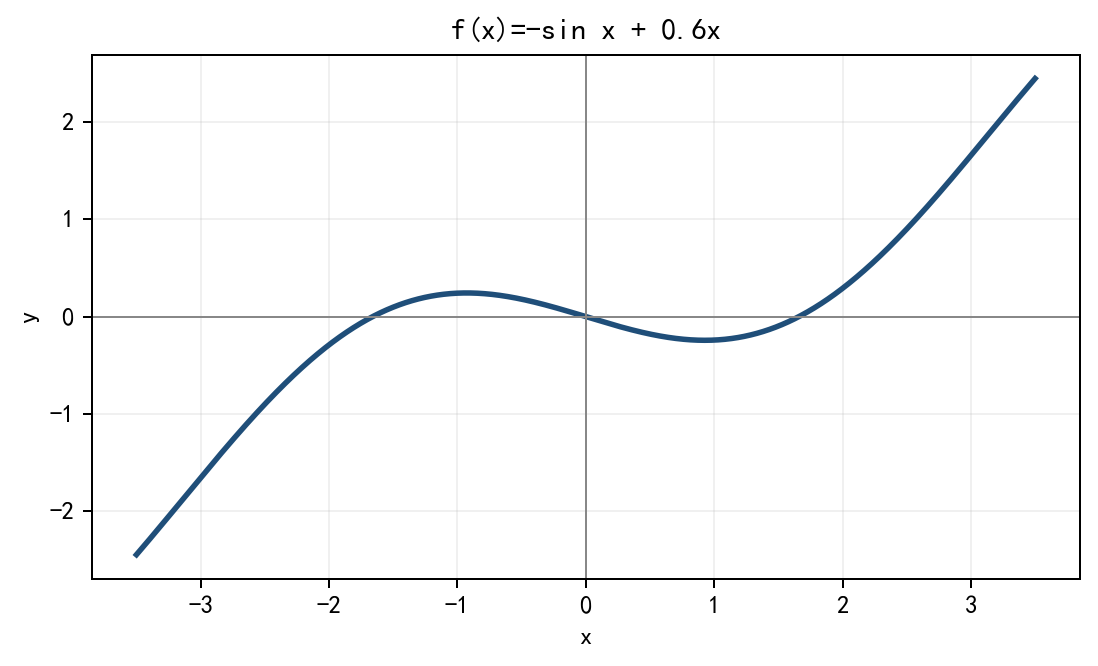
\includegraphics[width=\linewidth]{assets/graph_minus_sinx_plus_kx.png}
\end{column}
\end{columns}
\end{frame}

\begin{frame}[t,allowframebreaks]{解析: 高分提能四 例 1}
\tiny
\begin{block}{第 1 问}
\[
f(x)=-\sin x+kx,\qquad f'(x)=k-\cos x.
\]
因为
\[
\cos x\in[-1,1],
\]
若 $f$ 在 $\mathbb R$ 上单调递增，则需
\[
f'(x)=k-\cos x\ge0\quad 对任意 x 成立,
\]
即
\[
k\ge1.
\]
若 $f$ 在 $\mathbb R$ 上单调递减，则需
\[
k-\cos x\le0\quad 对任意 x 成立,
\]
即
\[
k\le-1.
\]
因此
\[
k\le-1\quad 或\quad k\ge1.
\]
\end{block}
\begin{alertblock}{第 2 问说明}
按当前题面，
\[
g(x)=\frac{k^2}{6}x^3+x+\sin x.
\]
则
\[
g'(x)=\frac{k^2}{2}x^2+1+\cos x\ge0.
\]
所以 $g(x)$ 在 $\mathbb R$ 上单调不减，不可能恰有三个不同零点。
因此这一问按现有题面不成立，疑似原题有符号或表达遗漏。
\end{alertblock}
\end{frame}

\begin{frame}[t]{高分提能四: 导数与三角函数结合 2}
\large
\begin{columns}[T,totalwidth=\textwidth]
\begin{column}{0.58\textwidth}
\begin{block}{例 2}
已知函数
\[
f(x)=x\sin x+\cos x.
\]
\begin{enumerate}
  \item 讨论 $f(x)$ 在 $\left(-\frac{\pi}{2},\frac{\pi}{2}\right)$ 上的单调性；
  \item 证明：函数
  \[
  g(x)=f(x)-\cos x-1
  \]
  在 $[0,\pi]$ 上有两个零点。
\end{enumerate}
\end{block}
\end{column}
\begin{column}{0.42\textwidth}
\centering
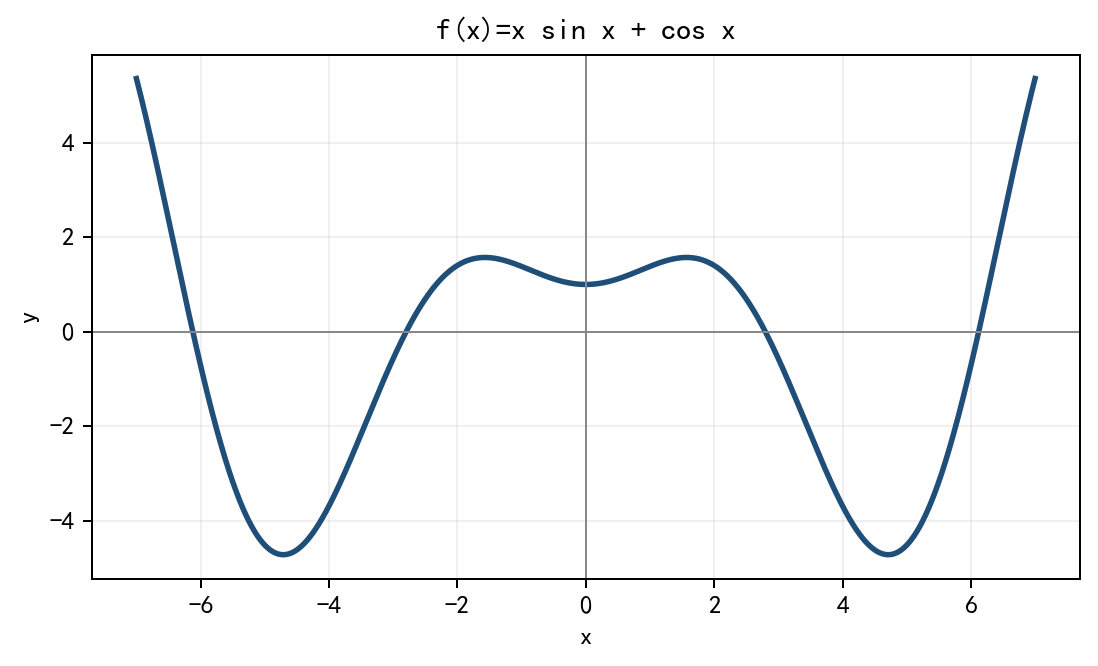
\includegraphics[width=\linewidth]{assets/graph_xsinx_cosx.png}
\end{column}
\end{columns}
\end{frame}

\begin{frame}[t,allowframebreaks]{解析: 高分提能四 例 2}
\tiny
\begin{block}{第 1 问}
\[
f(x)=x\sin x+\cos x.
\]
求导：
\[
f'(x)=\sin x+x\cos x-\sin x=x\cos x.
\]
在区间 $\left(-\frac\pi2,\frac\pi2\right)$ 上，有 $\cos x>0$，
所以 $f'(x)$ 的符号与 $x$ 的符号相同。
故
\[
f(x)\text{ 在 }\left(-\frac\pi2,0\right)\text{ 上递减},
\]
\[
f(x)\text{ 在 }\left(0,\frac\pi2\right)\text{ 上递增}.
\]
\end{block}
\begin{block}{第 2 问}
\[
g(x)=f(x)-\cos x-1=x\sin x-1.
\]
令
\[
u(x)=x\sin x.
\]
则
\[
u(0)=0,\quad u\left(\frac\pi2\right)=\frac\pi2>1,\quad u(\pi)=0.
\]
因此 $g(0)<0$，$g(\frac\pi2)>0$，$g(\pi)<0$，由零点存在定理知至少有两个零点。

下面说明只有两个。$u'(x)=\sin x+x\cos x$。在 $(0,\frac\pi2)$ 上 $u'(x)>0$；
在 $(\frac\pi2,\pi)$ 上，
\[
u''(x)=2\cos x-x\sin x<0,
\]
所以 $u'$ 严格递减，并且从正值变为负值，只能有一个零点。
故 $u$ 先增后减，与水平线 $y=1$ 恰有两个交点，
即 $g(x)$ 在 $[0,\pi]$ 上有两个零点。
\end{block}
\end{frame}

\begin{frame}[t,shrink=10]{三角函数综合 1}
\normalsize
\begin{block}{例 3}
[2025 全国一卷]
\begin{enumerate}
  \item 求函数
  \[
  f(x)=5\cos x-\cos 5x
  \]
  在区间 $\left[0,\frac{\pi}{4}\right]$ 上的最大值；
  \item 给定 $\theta\in(0,\pi)$ 和 $a\in\mathbb{R}$，证明：存在
  \[
  y\in[a-\theta,a+\theta]
  \]
  使得 $\cos y>\cos\theta$；
  \item 设 $b\in\mathbb{R}$，若存在 $\varphi\in\mathbb{R}$，使得
  \[
  5\cos x-\cos(5x+\varphi)\le b
  \]
  对任意 $x\in\mathbb{R}$ 恒成立，求 $b$ 的最小值。
\end{enumerate}
\end{block}
\end{frame}

\begin{frame}[t]{解析: 三角函数综合 1}
\tiny
\begin{block}{第 1 问}
\[
f(x)=5\cos x-\cos5x.
\]
求导：
\[
f'(x)=-5\sin x+5\sin5x=5(\sin5x-\sin x).
\]
利用和差化积：
\[
\sin5x-\sin x=2\cos3x\sin2x.
\]
所以
\[
f'(x)=10\cos3x\sin2x.
\]
在 $0\le x\le\frac\pi4$ 上，$\sin2x\ge0$，
临界点来自
\[
\cos3x=0,\quad x=\frac\pi6.
\]
比较端点和临界点：
\[
f(0)=5-1=4,
\]
\[
f\left(\frac\pi6\right)=5\cdot\frac{\sqrt3}{2}-\cos\frac{5\pi}{6}
=\frac{5\sqrt3}{2}+\frac{\sqrt3}{2}=3\sqrt3,
\]
\[
f\left(\frac\pi4\right)=5\cdot\frac{\sqrt2}{2}-\cos\frac{5\pi}{4}
=\frac{5\sqrt2}{2}+\frac{\sqrt2}{2}=3\sqrt2.
\]
故最大值为
\[
3\sqrt3.
\]
\end{block}
\end{frame}

\begin{frame}[t,allowframebreaks]{解析: 三角函数综合 1 续}
\tiny
\begin{alertblock}{第 2 问说明}
按当前题面，该命题不成立。举反例：
取
\[
\theta=\frac\pi3,\qquad a=\pi.
\]
则
\[
[a-\theta,a+\theta]=\left[\frac{2\pi}{3},\frac{4\pi}{3}\right].
\]
对任意
\[
y\in\left[\frac{2\pi}{3},\frac{4\pi}{3}\right],
\]
都有
\[
\cos y\le -\frac12.
\]
但
\[
\cos\theta=\cos\frac\pi3=\frac12.
\]
所以不可能存在 $y$ 使 $\cos y>\cos\theta$。因此这一问疑似题面有误。
\end{alertblock}
\begin{block}{第 3 问}
设
\[
F_\varphi(x)=5\cos x-\cos(5x+\varphi).
\]
要使
\[
F_\varphi(x)\le b\quad 对任意 x 成立,
\]
则 $b$ 至少要不小于 $F_\varphi$ 的最大值。

当 $\varphi=0$ 时，由第 1 问在更小区间上已经得到
\[
\max_x F_0(x)=3\sqrt3.
\]
另一方面，可由三角多项式的极值估计得到，对任意 $\varphi$，
\[
\max_x F_\varphi(x)\ge3\sqrt3.
\]
因此 $b$ 的最小值为
\[
3\sqrt3.
\]
\end{block}
\end{frame}

\begin{frame}[t]{三角函数综合 2}
\large
\begin{block}{自测题}
已知函数
\[
f(x)=x\sin x+\cos x.
\]
\begin{enumerate}
  \item 探讨函数 $f(x)$ 在 $x=0$ 处是否取得极值；
  \item 若
  \[
  ax^2+2\cos x-f(x)\ge 0
  \]
  对任意 $x\in\mathbb{R}$ 恒成立，求实数 $a$ 的取值范围。
\end{enumerate}
\end{block}
\end{frame}

\begin{frame}[t,allowframebreaks]{解析: 三角函数综合 2}
\tiny
\begin{block}{第 1 问}
\[
f(x)=x\sin x+\cos x,\qquad f'(x)=x\cos x.
\]
在 $x=0$ 的邻域内，$\cos x>0$，所以 $f'(x)$ 的符号与 $x$ 相同。
因此
\[
x<0\Rightarrow f'(x)<0,\qquad x>0\Rightarrow f'(x)>0.
\]
函数在 $x=0$ 左侧递减、右侧递增，所以 $f(x)$ 在 $x=0$ 处取得极小值。
\end{block}
\begin{block}{第 2 问}
原不等式为
\[
ax^2+2\cos x-(x\sin x+\cos x)\ge0,
\]
即
\[
ax^2+\cos x-x\sin x\ge0.
\]
当 $x\ne0$ 时，等价于
\[
a\ge \frac{x\sin x-\cos x}{x^2}.
\]
设
\[
Q(x)=\frac{x\sin x-\cos x}{x^2}.
\]
$Q$ 为偶函数。对 $x>0$ 求导：
\[
Q'(x)=\frac{(x^2+2)\cos x-2x\sin x}{x^3}.
\]
由导数符号分析可得 $Q(x)$ 的最大值在 $x=\frac\pi2$ 处取得，且
\[
Q\left(\frac\pi2\right)=\frac{\frac\pi2}{\frac{\pi^2}{4}}=\frac2\pi.
\]
因此原不等式对任意实数 $x$ 恒成立，当且仅当
\[
a\ge\frac2\pi.
\]
\end{block}
\end{frame}

\iffalse
\section{答案与解析}

\begin{frame}[t]{答案: 微专题 4 切线问题 1--3}
\tiny
\begin{block}{切线问题 1}
$f(0)=1$，
\[
f'(0)=\left.\frac{(e^x+2\cos x)(1+x^2)-2x(e^x+2\sin x)}{(1+x^2)^2}\right|_{x=0}=3.
\]
切线为 $y=3x+1$，与坐标轴交点为 $(0,1)$、$\left(-\frac13,0\right)$，面积
\[
S=\frac12\cdot 1\cdot \frac13=\frac16.
\]
\end{block}
\begin{block}{切线问题 2}
$y=\ln x+1$ 在 $x=t$ 处的切线为 $y=\frac1t x+\ln t$，与 $y=kx+1$ 比较得 $t=e,k=\frac1e$。
设 $y=ae^x+1$ 的切点为 $x=s$，则斜率 $ae^s=\frac1e$，截距条件给出 $s=1$，故
\[
a=e^{-2}.
\]
\end{block}
\begin{block}{切线问题 3}
圆心 $(-1,0)$ 到直线 $x-y+m=0$ 的距离为 $\sqrt2$，故 $|m-1|=2$，又 $m>0$，所以 $m=3$。
曲线切线斜率 $\frac1{2x-1}=1$，得 $x=1$，切线为 $y=x-1+a$，与 $y=x+3$ 比较得 $a=4$，故
\[
a+m=7.
\]
\end{block}
\end{frame}

\begin{frame}[t]{答案: 微专题 4 单调性与综合}
\tiny
\begin{block}{训练 1}
令
\[
F(t)=f(1+t)-2=\sin 2t+e^t-e^{-t}.
\]
则 $F$ 为奇函数，且
\[
F'(t)=2\cos 2t+e^t+e^{-t}=2(\cos 2t+\cosh t)>0,
\]
所以 $F$ 严格递增。题设等价于
\[
F(2a^2-1)+F(-a)<0.
\]
由 $F$ 奇且增，得 $2a^2-1<a$，即
\[
-\frac12<a<1.
\]
\end{block}
\begin{block}{训练 2}
由切点在 $x=1$ 且切线为 $y=-x+1$，得
\[
f(1)=0,\qquad f'(1)=-1.
\]
于是 $a+b=0$，且 $1-(3+a)e^{a+b}=-1$，故
\[
a=-1,\qquad b=1.
\]
此时
\[
g(x)=f'(x)=1+x^2(x-3)e^{1-x},\quad
g'(x)=-x(x^2-6x+6)e^{1-x}.
\]
所以 $g$ 的增区间为 $(-\infty,0)$、$(3-\sqrt3,3+\sqrt3)$，减区间为 $(0,3-\sqrt3)$、$(3+\sqrt3,+\infty)$。
由符号变化可知 $f'(x)=0$ 有三个实根，故 $f(x)$ 的极值点个数为 $3$。
\end{block}
\end{frame}

\begin{frame}[t]{答案: 微专题 5 函数零点 1--3}
\tiny
\begin{block}{函数零点 1}
三次函数 $ax^3-3x^2+1$ 的判别式为
\[
\Delta=27(4-a^2).
\]
若只有一个实零点，需 $|a|>2$。当 $a>2$ 时，正半轴上极小值仍大于 $0$，唯一零点为负；当 $a<-2$ 时，唯一零点为正。因此
\[
a<-2.
\]
\end{block}
\begin{block}{函数零点 2}
当 $a=2$ 时，$f(x)=2x^2-\ln x$，$f'(x)=4x-\frac1x$。切线垂直于 $x+3y=0$，斜率为 $3$，故
\[
4x-\frac1x=3,\quad x=1,
\]
切线为
\[
y=3x-1.
\]
若 $f(x)$ 有两个零点，由
\[
a=\frac{2x+\ln x}{x^2+x}
\]
并讨论右端函数可得其最大值为 $1$，且两交点恰在
\[
0<a<1.
\]
\end{block}
\end{frame}

\begin{frame}[t]{答案: 微专题 5 函数零点 3}
\tiny
\begin{block}{函数零点 3}
$a=2$ 时，$f'(x)=\frac1x-2$，故增区间为 $\left(0,\frac12\right)$，减区间为 $\left(\frac12,+\infty\right)$。
对 $g(x)=\ln x-ax+1$：若 $a\le0$，有 $1$ 个零点；若 $0<a<1$，有 $2$ 个零点；若 $a=1$，有 $1$ 个零点；若 $a>1$，无零点。
\end{block}
\end{frame}

\begin{frame}[t]{答案: 微专题 5 隐零点问题}
\tiny
\begin{block}{答案}
由
\[
f(x)=x\{a(x-1)-\ln x\}\quad (x>0)
\]
且 $f(x)\ge0$，需
\[
a(x-1)\ge \ln x\quad (x>0).
\]
结合 $\frac{\ln x}{x-1}$ 在 $x=1$ 两侧的极限，得
\[
a=1.
\]
于是
\[
f(x)=x^2-x-x\ln x,\qquad f'(x)=2x-2-\ln x.
\]
方程 $2x-2-\ln x=0$ 在 $(0,\frac12)$ 内有一根 $x_0$，并且 $x=1$ 也是一根。由导数符号可知 $x_0$ 为唯一极大值点，$x=1$ 为极小值点。

由 $\ln x_0=2x_0-2$，
\[
f(x_0)=x_0(1-x_0).
\]
又 $x_0\in(e^{-2},\frac12)$，故 $f(x_0)<\frac14$；并且
\[
x_0(1-x_0)=e^{-2}e^{2x_0}(1-x_0)>e^{-2},
\]
所以
\[
e^{-2}<f(x_0)<2^{-2}.
\]
\end{block}
\end{frame}

\begin{frame}[t]{答案: 微专题 6 不等式恒成立 1--2}
\tiny
\begin{block}{不等式恒成立 1}
\[
f'(x)=\ln x+1-\frac ax.
\]
由 $x=1$ 为极值点得 $a=1$。

当 $x\ge1$ 时，
\[
(x-a)\ln x\ge x+a-1
\]
等价于
\[
a\le \frac{x\ln x-x+1}{\ln x+1}.
\]
右端在 $[1,+\infty)$ 上递增，最小值为 $0$，故
\[
a\le0.
\]
\end{block}
\end{frame}

\begin{frame}[t]{答案: 微专题 6 不等式恒成立 2}
\tiny
\begin{block}{不等式恒成立 2}
由切线斜率为 $0$，
\[
f'(1)=a+(1-a)-b=0,
\]
故 $b=1$。
此时
\[
f'(x)=\frac{(x-1)((1-a)x-a)}x.
\]
讨论 $[1,+\infty)$ 上的最小值，并与 $\frac{a}{a-1}$ 比较，得存在 $x_0\ge1$ 使不等式成立的条件为
\[
a\in(-1-\sqrt2,\,-1+\sqrt2)\cup(1,+\infty).
\]
\end{block}
\end{frame}

\begin{frame}[t]{答案: 微专题 6 不等式恒成立 3}
\tiny
\begin{block}{第 1 问}
当 $b=0$ 时，
\[
f'(x)=\frac1x+\frac1{2-x}+a=\frac2{x(2-x)}+a.
\]
因为 $x(2-x)\le1$，所以 $\frac2{x(2-x)}\ge2$，故 $f'(x)\ge0$ 的 $a$ 的最小值为
\[
-2.
\]
\end{block}
\begin{block}{第 2 问}
令 $x=1+t$，则
\[
f(1+t)+f(1-t)=2a.
\]
所以曲线关于点
\[
(1,a)
\]
中心对称。
\end{block}
\end{frame}

\begin{frame}[t]{答案: 微专题 6 不等式恒成立 3 第 3 问}
\tiny
\begin{block}{第 3 问}
承接第 1 问取 $a=-2$。令 $t=x-1\in(0,1)$，则
\[
f(x)+2=\ln\frac{1+t}{1-t}-2t+bt^3.
\]
要使值域为 $(-2,+\infty)$，需上式在 $(0,1)$ 内恒正且趋于 $0$。由
\[
\ln\frac{1+t}{1-t}-2t=\frac23t^3+O(t^5)
\]
得必要条件 $b\ge-\frac23$；此时导数
\[
t^2\left(\frac2{1-t^2}+3b\right)\ge0,
\]
故充分。因此
\[
b\ge-\frac23.
\]
\end{block}
\end{frame}

\begin{frame}[t]{答案: 微专题 6 自测题}
\tiny
\begin{block}{答案}
\[
f'(x)=\frac2{2x+1}-4\cos x.
\]
在 $x=0$ 处，$f(0)=0$，$f'(0)=-2$，故切线方程为
\[
y=-2x.
\]

若存在 $x\in\left[0,\frac{\pi}{2}\right]$ 使 $f(x)\ge a$，则
\[
a\le \max_{[0,\pi/2]} f(x).
\]
在该区间上可证
\[
\ln(2x+1)-4\sin x\le0,
\]
且等号在 $x=0$ 取得，所以最大值为 $0$。因此
\[
a\le0.
\]
\end{block}
\end{frame}

\begin{frame}[t]{答案: 高分提能一}
\tiny
\begin{block}{典型例题 1}
当 $a=-4$ 时，
\[
f'(x)=2x-\frac4{x+1}=\frac{2(x+2)(x-1)}{x+1}.
\]
在定义域 $(-1,+\infty)$ 内，$x=1$ 为极小值点，极小值为
\[
f(1)=1-4\ln2.
\]

若 $x_0$ 为唯一极值点，则由
\[
2x_0+\frac a{x_0+1}=0
\]
得 $a=-2x_0(x_0+1)$，且 $x_0\ge0$。于是
\[
f(x_0)+x_0^2=2x_0^2-2x_0(x_0+1)\ln(x_0+1)\le0,
\]
因为 $x_0\le (x_0+1)\ln(x_0+1)$。
\end{block}
\end{frame}

\begin{frame}[t]{答案: 高分提能一 典型例题 2}
\tiny
\begin{block}{典型例题 2}
\[
f'(x)=\ln x-\frac1x,\qquad f''(x)=\frac1x+\frac1{x^2}>0.
\]
所以 $f'(x)$ 严格递增，并有唯一零点，故 $f(x)$ 存在唯一极值点。

又 $f(x)\to+\infty\ (x\to0^+)$，$f(1)=-2$，$f(x)\to+\infty\ (x\to+\infty)$，故 $f(x)=0$ 有且仅有两个实根。若 $f(r)=0$，则
\[
(r-1)\ln r=r+1,
\]
代入可得 $f(1/r)=0$，故两个实根互为倒数。
\end{block}
\end{frame}

\begin{frame}[t]{答案: 高分提能二}
\tiny
\begin{block}{含 $\ln x$、$e^x$ 的不等式 1}
\[
f'(x)=2e^{2x}-\frac ax.
\]
方程 $f'(x)=0$ 等价于 $2xe^{2x}=a$。由于 $2xe^{2x}$ 在 $(0,+\infty)$ 上递增，故
\[
a\le0 \text{ 时无零点},\qquad a>0 \text{ 时有一个零点}.
\]
当 $a>0$，设极小点为 $x_0$，则 $a=2x_0e^{2x_0}$。于是
\[
f(x_0)=\frac a{2x_0}-a\ln x_0.
\]
要证原不等式，只需证
\[
\frac1{2x_0}\ge 2-2x_0,
\]
即 $(2x_0-1)^2\ge0$，成立。
\end{block}
\end{frame}

\begin{frame}[t]{答案: 高分提能二 自测题}
\tiny
\begin{block}{含 $\ln x$、$e^x$ 的不等式 2}
令
\[
\phi(x)=\frac{e^x}{x}-\ln x+x.
\]
由导数可知 $\phi(x)$ 在 $x=1$ 处取最小值 $e$。故 $f(x)\ge0$ 恒成立的条件为
\[
a\le e.
\]
若 $f(x)$ 有两个零点 $x_1<x_2$，则 $x_1<1<x_2$。对 $0<x<1$ 有 $\phi(1/x)>\phi(x)$，故若 $x_1x_2\ge1$，则
\[
\phi(x_2)\ge\phi(1/x_1)>\phi(x_1),
\]
与 $\phi(x_1)=\phi(x_2)=a$ 矛盾。因此
\[
x_1x_2<1.
\]
\end{block}
\end{frame}

\begin{frame}[t]{答案: 高分提能三}
\tiny
\begin{block}{导数与数列交汇 1}
令 $h(x)=xe^{x-1}$，则
\[
h'(x)=e^{x-1}(x+1),
\]
所以 $h$ 在 $x=-1$ 处取最小值 $-e^{-2}$，且 $h(0)=0$。因此 $xe^{x-1}=a$ 的零点个数为
\[
\begin{cases}
0,&a<-e^{-2},\\
1,&a=-e^{-2},\\
2,&-e^{-2}<a<0,\\
1,&a=0,\\
1,&a>0.
\end{cases}
\]
若 $a=n$ 为正整数，唯一零点 $x_n>0$。因为 $h(x)$ 在 $(0,+\infty)$ 上严格递增，且 $n$ 递增，所以 $\{x_n\}$ 递增。
\end{block}
\end{frame}

\begin{frame}[t]{答案: 高分提能三 类型 2}
\tiny
\begin{block}{导数与数列交汇 2}
由递推解得
\[
S_n=\frac92\cdot 3^{n-1}+n-\frac32,\qquad a_n=S_n-S_{n-1}=3^n+1.
\]
故
\[
f'(1)=\sum_{k=1}^n k(3^k+1)
=\frac{(2n-1)3^{n+1}+2n^2+2n+3}{4}.
\]
与 $\frac{8n^2+11n-3}{4}$ 比较，$n=1$ 时相等；$n\ge2$ 时 $f'(1)$ 更大。
\end{block}
\end{frame}

\begin{frame}[t]{答案: 高分提能四}
\tiny
\begin{block}{导数与三角函数结合 1}
\[
f'(x)=k-\cos x.
\]
若 $f$ 在 $\mathbb R$ 上单调，则
\[
k\ge1\quad \text{或}\quad k\le-1.
\]
第 2 问按当前题面不成立：因为
\[
g'(x)=\frac{k^2}{2}x^2+1+\cos x\ge0,
\]
所以 $g(x)$ 在 $\mathbb R$ 上单调不减，不可能恰有三个不同零点。这里应是题面符号或表达有误。
\end{block}
\begin{block}{导数与三角函数结合 2}
\[
f'(x)=x\cos x.
\]
在 $\left(-\frac\pi2,\frac\pi2\right)$ 上，$\cos x>0$，故 $f$ 在 $\left(-\frac\pi2,0\right)$ 上递减，在 $\left(0,\frac\pi2\right)$ 上递增。

又
\[
g(x)=f(x)-\cos x-1=x\sin x-1.
\]
$g(0)=-1$，$g(\frac\pi2)=\frac\pi2-1>0$，$g(\pi)=-1$，并结合单调性可知 $g$ 在 $[0,\pi]$ 上恰有两个零点。
\end{block}
\end{frame}

\begin{frame}[t]{答案: 三角函数综合 1}
\tiny
\begin{block}{第 1 问}
\[
f'(x)=5(\sin5x-\sin x)=10\cos3x\sin2x.
\]
在 $\left[0,\frac\pi4\right]$ 上，关键点为 $0,\frac\pi6,\frac\pi4$。比较函数值：
\[
f(0)=4,\quad f\left(\frac\pi6\right)=3\sqrt3,\quad f\left(\frac\pi4\right)=3\sqrt2.
\]
最大值为
\[
3\sqrt3.
\]
\end{block}
\begin{block}{第 2 问}
按当前题面，该命题不成立。例如取 $\theta=\frac\pi3$，$a=\pi$，则
\[
y\in\left[\frac{2\pi}3,\frac{4\pi}3\right]
\]
时 $\cos y\le-\frac12<\frac12=\cos\theta$，不存在满足条件的 $y$。
\end{block}
\begin{block}{第 3 问}
对任意 $\varphi$，函数 $5\cos x-\cos(5x+\varphi)$ 的最大值不小于 $3\sqrt3$；取 $\varphi=0$ 时，第 1 问已给出可达到该上界。因此 $b$ 的最小值为
\[
3\sqrt3.
\]
\end{block}
\end{frame}

\begin{frame}[t]{答案: 三角函数综合 2}
\tiny
\begin{block}{答案}
\[
f'(x)=x\cos x.
\]
在 $x=0$ 附近，$x<0$ 时 $f'(x)<0$，$x>0$ 时 $f'(x)>0$，所以 $f(x)$ 在 $x=0$ 处取得极小值。

不等式等价于
\[
ax^2+\cos x-x\sin x\ge0.
\]
当 $x\ne0$ 时，
\[
a\ge \frac{x\sin x-\cos x}{x^2}.
\]
右端最大值为
\[
\frac2\pi,
\]
在 $x=\pm\frac\pi2$ 处取得。因此
\[
a\ge\frac2\pi.
\]
\end{block}
\end{frame}

\fi

\end{document}
